\begin{comment}
    

\documentclass[lang=cn,10pt,green]{elegantbook} 
\title{2025年数理经济学笔记}
\subtitle{授课: 杨佳楠老师}

\author{徐靖}
\institute{PKU}
\date{Febuary 27, 2025}
\bioinfo{声明}{请勿用于个人学习外其他用途!}

\extrainfo{个人笔记, 如有谬误, 欢迎指正! 联系方式 : 2200012917@stu.pku.edu.cn}

\setcounter{tocdepth}{3}

\logo{pkuhub.cn.png}
\cover{cover.jpg}


% 本文档命令
\usepackage{array}
\newcommand{\ccr}[1]{\makecell{{\color{#1}\rule{1cm}{1cm}}}}

% 修改标题页的橙色带
% \definecolor{customcolor}{RGB}{32,178,170}
% \colorlet{coverlinecolor}{customcolor}

\begin{document}

\maketitle
\frontmatter

\tableofcontents

\mainmatter
% \end{comment}
% TODO

\chapter{Multi-Variable Unconstrained Optimization}

\begin{introduction}[Keywords]
    \item First Order Condition 一阶条件
    \item Bisection Method 二分法
    \item Secant Method 割线法
    \item False Position Method 假位法
    \item Newton's Method 牛顿法
\end{introduction}

\section{First Order Condition}
An Unconstrained Optimization Problem is :
$$\min_{x \in \mathbb{R}^n} f(x)$$

\begin{definition}
    \textbf{First Order Condition (FOC)}:  $\nabla f(x^*) = 0$.
    \begin{itemize}
        \item $x^*$ is a \textbf{stationary point} (驻点) of $f$.
        \item It is necessary but not sufficient.
    \end{itemize}
    \textbf{global minimum}: $f(x^*) \leq f(x)$ for all $x \in \mathbb{R}^n$.
    
    \textbf{local minimum}: $f(x^*) \leq f(x)$ for all $x \in B(x^*, \epsilon)$ for some $\epsilon > 0$.
\end{definition}

\begin{proposition}
    Let $f: \mathbb{R}^n \to \mathbb{R}$ be a continuously differentiable function, and $\nabla f(x^*) = 0$. If $\nabla^2 f(x^*)$ is:
    \begin{itemize}
        \item positive definite, then $x^*$ is a local minimum.
        \item negative definite, then $x^*$ is a local maximum.
        \item indefinite, then $x^*$ is a \textbf{saddle point}. (鞍点)
    \end{itemize} 
\end{proposition}

\section{Convex Optimization}
\begin{definition}[Convex Function]
    A function $f: \mathbb{R}^n \to \mathbb{R}$ is convex if for all $x, y \in \mathbb{R}^n$ and $\lambda \in [0, 1]$:
    $$f(\lambda x + (1 - \lambda) y) \leq \lambda f(x) + (1 - \lambda) f(y)$$
\end{definition}
\begin{theorem}
    A twice continuously differentiable function $f: \mathbb{R}^n \to \mathbb{R}$ is convex if and only if its Hessian matrix $\nabla^2 f(x)$ is positive semidefinite for all $x \in \mathbb{R}^n$.
\end{theorem}

\begin{proposition}
    Let $f$ be differentiable. Then $f$ is (strictly) convex if and only if:
    $$ f(y) - f(x) (>) \geq \nabla f(x) \cdot (y - x) $$
    for all $x, y \in \mathbb{R}^n$.
\end{proposition}
\begin{theorem}[Minimum/maximum Characterization]
    Let $f: \mathbb{R}^n \to \mathbb{R}$ be a convex (concave) function. Then $x^*$ is a local minimum (maximum) if and only if:
    $$\nabla f(x^*) = 0$$
    \begin{itemize}
        \item If $f$ is strictly \textbf{convex}, then $x^*$ is a global minimum.
        \item If $f$ is strictly \textbf{concave}, then $x^*$ is a global maximum.
    \end{itemize}
\end{theorem}
\section{Numerical Optimization}
\subsection{Bisection Method}
\begin{definition}[Bisection Method]
    A simple, robust method for finding roots of continuous functions on bounded intervals
    \begin{itemize}
        \item Start with an interval $[a, b]$ such that $f(a)f(b) < 0$.
        \item Compute the midpoint $c = \frac{a + b}{2}$, and evaluate $f(c)$.
        \item Replace $a$ or $b$ with $c$ based on the sign of $f(c)$.
        \item Iterate until desired precision.
    \end{itemize}
\end{definition}
\begin{definition}[Convergence Rate and Order 收敛速度和阶]
    For iteration $x_n$ approaching the root $r$, the convergence rate $C$ and order $\rho$ are defined as: 
    $$\lim_{n \to \infty} \frac{|x_{n+1} - r|}{|x_n - r|^\rho} = C$$
    \begin{itemize}
        \item Linear convergence: $\rho = 1$, $C < 1$.
        \item Quadratic convergence: $\rho = 2$, $C < 1$.
        \item Superlinear convergence: $\rho > 1$, $C < 1$.
    \end{itemize}
\end{definition}

\begin{table}[htbp]
    \centering
    \begin{tabularx}{\textwidth}{|l|X|c|c|}
        \hline
        \textbf{Method} & \textbf{Definition} & \textbf{Rate} & \textbf{Order} \\
        \hline
        Bisection & 
        \makecell[l]{Iteratively bisects an interval \\ and selects a subinterval} 
        & Linear ($C = 0.5$) & 1 \\
        \hline
        Secant & 
        \makecell[l]{Root approximation via secant line \\ through two points} 
        & Superlinear ($C \approx 1.618$) & 1.618 \\
        \hline
        False Position & 
        \makecell[l]{Bisection variant with \\ linear interpolation updates} 
        & Linear & 1 \\
        \hline
        Newton-Raphson & 
        \makecell[l]{Derivative-based iterative \\ root-finding} 
        & Quadratic ($C \propto f''$) & 2 \\
        \hline
        Gradient method & 
        \makecell[l]{Function minimization via \\ negative gradient direction} 
        & Linear ($C \propto \kappa$) & 1 \\
        \hline
    \end{tabularx}
    \caption{Compact Comparison of Numerical Methods}
    \label{tab:comparison_compact}
\end{table}
\begin{definition}[Methods]
    \textbf{Secant Method}:
    \begin{itemize}
        \item Compute the secant line through $(x_0, f(x_0))$ and $(x_1, f(x_1))$.
        \item Find the intersection with the x-axis to get the next approximation $x_2$.
        \item Iterate until convergence.
    \end{itemize}
    \begin{equation}
        x_{n+1} = x_n - \frac{f(x_n)(x_n - x_{n-1})}{f(x_n) - f(x_{n-1})}   
    \end{equation}
    \textbf{False Position Method}:
    \begin{itemize}
        \item Similar to the secant method, but always keeps the interval $[a, b]$ such that $f(a)f(b) < 0$.
        \item Update $a$ or $b$ based on the sign of $f(c)$.
        \item Iterate until convergence.
    \end{itemize}
    $$
    \begin{aligned}
        c &= \frac{a f(b) - b f(a)}{f(b) - f(a)}, \\
        [a, b] &\gets [a, c] \quad \text{if} \quad f(a)f(c) < 0, \\
        [a, b] &\gets [c, b] \quad \text{if} \quad f(b)f(c) < 0.
    \end{aligned}
    $$
\end{definition}

% 并排放入两张图片
\begin{figure}
    \centering
    \begin{minipage}{0.45\textwidth}
        \centering
        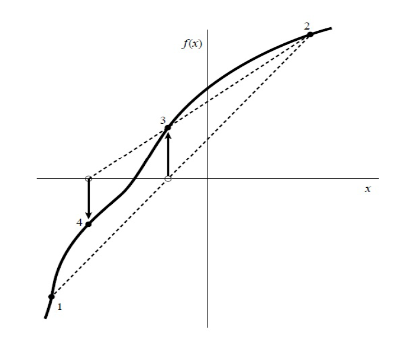
\includegraphics[width=\textwidth]{image/secantmethod.png}
        \caption{Secant Method}
        \label{fig:secantmethod}
    \end{minipage}\hfill
    \begin{minipage}{0.45\textwidth}
        \centering
        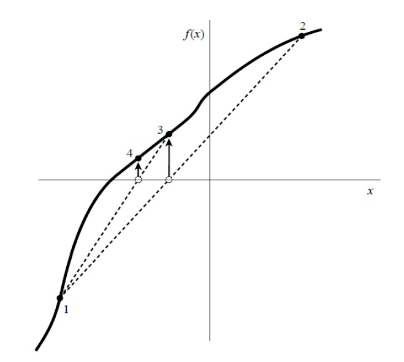
\includegraphics[width=\textwidth]{image/falsepositionmethod.png}
        \caption{False Position Method}
        \label{fig:falsepositionmethod}
    \end{minipage}
\end{figure}
\begin{note}
若初始值足够接近根且函数光滑, 则Secant Method 收敛速度优于False Position Method, 但可能因迭代点跳出根的邻域而发散. False Position Method 保证收敛, 但多一个异号的初始条件且速度较慢.
\end{note}
\begin{definition}[Newton-Raphson Method]
    \begin{itemize}
        \item Start with an initial guess $x_0$.
        \item Compute the next approximation using the formula:
        $$x_{n+1} = x_n - \frac{f(x_n)}{f'(x_n)}$$
        \item Iterate until convergence.
    \end{itemize}
\end{definition}
\begin{problem}
为什么牛顿法是二阶收敛的?
\end{problem}
\begin{solution}
对 $f(x)$ 在 $x_n$ 处做泰勒展开, 对于 $f(r)=0$:
$$f(r) = f(x_n) + f'(x_n)(r - x_n) + \frac{f''(x_n)}{2}(r - x_n)^2 + O((x - x_n)^3)$$
带入牛顿法迭代公式 $x_{n+1} = x_n - \frac{f(x_n)}{f'(x_n)}$:
$$x_{n+1} - r = (x_n - r)^2 \cdot \frac{f''(x_n)}{2f'(x_n)} $$
\end{solution}
\begin{note}
牛顿法初期可能出问题, 如果不满足足够接近根的假设.

牛顿法可以很好地应用到多变量上, 但过程中Hessian矩阵的逆矩阵计算量较大, 并且他是一个 local method.
\end{note}
\begin{example}
    将牛顿法应用到求解二次可微函数的极值问题, 可以求解 first order condition:
    $$ x_{n+1} = x_n - [\nabla^2 f(x_n)]^{-1} \nabla f(x_n) $$
\end{example}

\begin{definition}[Gradient Method]
    \begin{itemize}
        \item Start with an initial guess $x_0$ and error tolerance $\epsilon$.
        \item Iterate until $\|x_{n+1} - x_n\| < \epsilon$:
        \begin{itemize}
            \item Compute the gradient $\nabla f(x_n)$.
            \item Define $\phi(t) = f(x_n - t \nabla f(x_n))$.
            \item Find the minimum of $\phi(t)$ using a one-variable optimization method (e.g., bisection, secant, or Newton's method).
            \item Defint $x_{n+1} = x_n - t^* \nabla f(x_n)$.
        \end{itemize}
    \end{itemize}
\end{definition}

%\end{document}







